\chapter{Architecture applicative logique proposée}
\section{Objectif}
L'architecture applicative logique traduit la cible fonctionnelle en composants logiciels sans imposer une stack définitive. Elle sert à préparer une future implémentation tout en respectant le périmètre du stage : conception, modélisation et validation.

\begin{figure}[H]
\centering
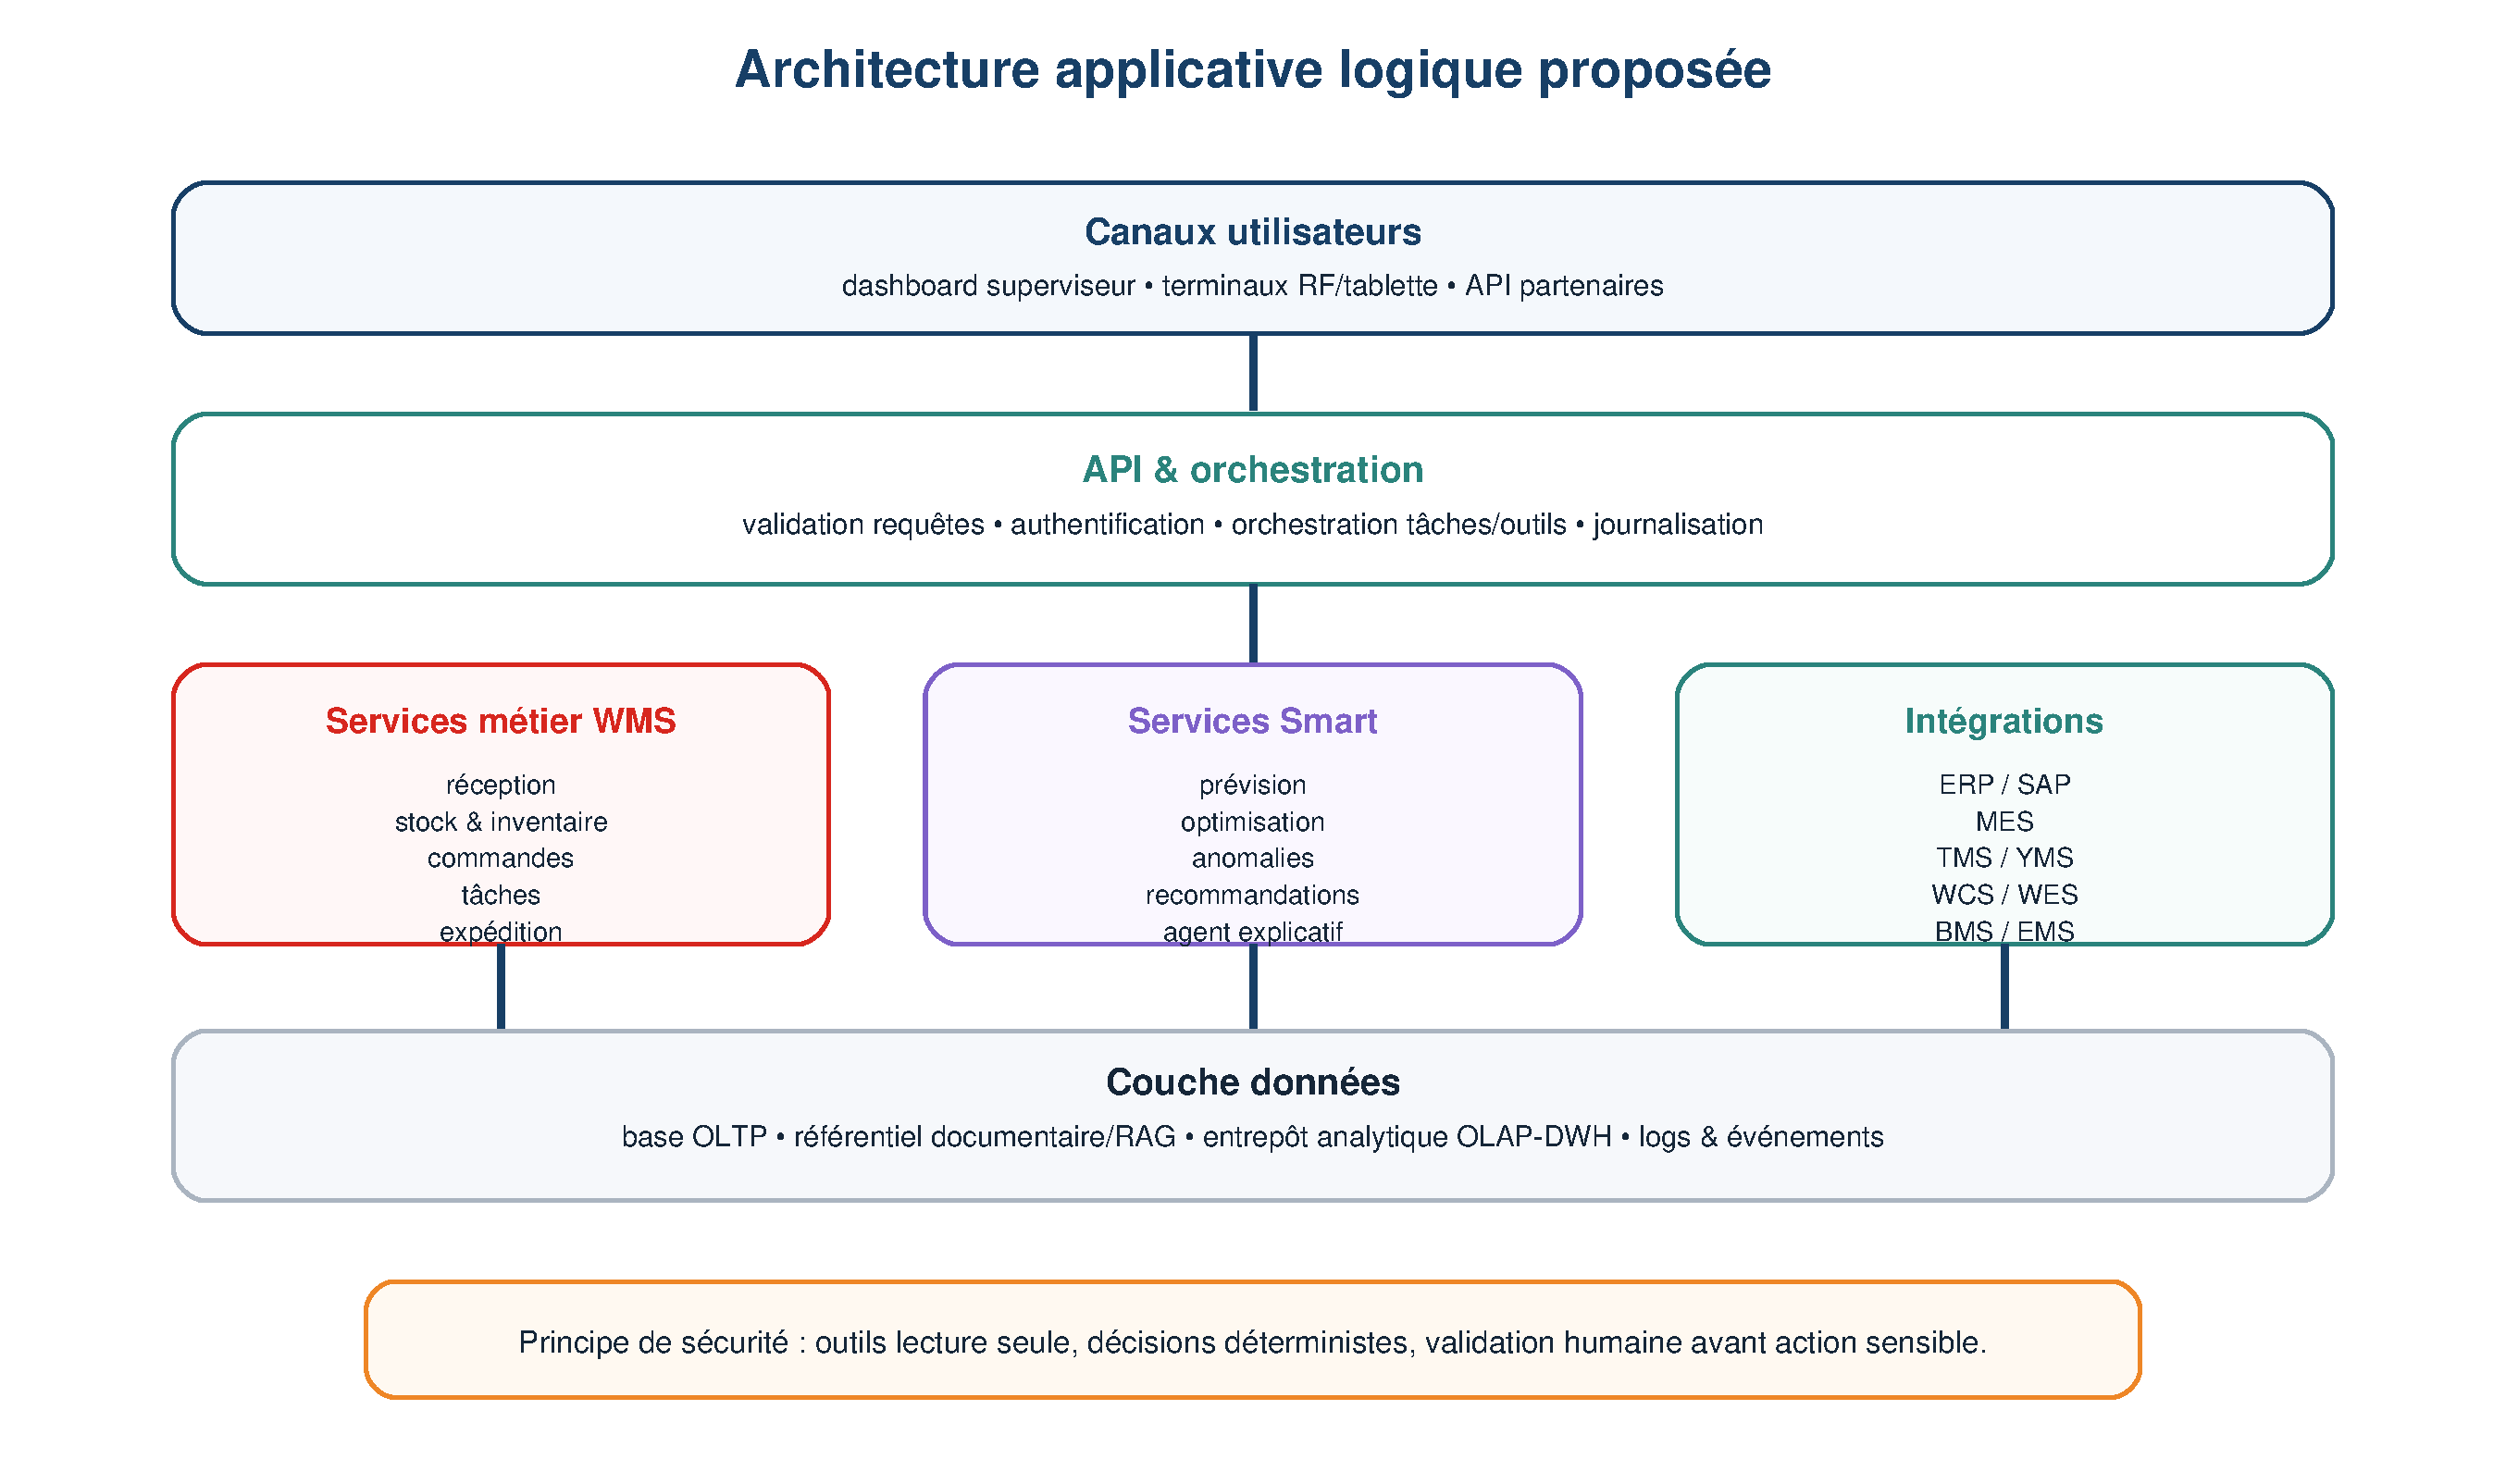
\includegraphics[width=0.94\linewidth]{figures/chapitre6/architecture_applicative_logique.pdf}
\caption{Architecture applicative logique proposée pour le Smart WMS.}
\label{fig:architecture-applicative}
\end{figure}

\section{Positionnement du prototype SmartWMS AI Operations Agent}
Le dépôt local SmartWMS AI Operations Agent illustre une partie de cette architecture : une interface Next.js, une API FastAPI, un runner d'agent, des outils WMS en lecture seule, un moteur de décisions déterministes et un retriever de documents synthétiques. Cette maquette ne constitue pas un WMS complet. Elle démontre surtout comment une couche d'aide à la décision peut consommer des faits structurés sans inventer la logique métier.

\section{Principes de sûreté}
Les règles de décision doivent rester testables hors du modèle de langage. Dans la maquette, les calculs de disponibilité, position de stock, demande ouverte, risque de rupture, priorité de réapprovisionnement et quantité de réapprovisionnement sont centralisés dans un service métier déterministe. Le modèle de langage explique les résultats ; il ne crée pas de mouvements de stock et ne prend pas de décision d'achat autonome.
